\chapter{De la mécanique Lagrangienne aux théories de la physique moderne}
    \chapterprecishere{
        ``Quand je dis que Rome est à la cité ce que le chèvre est au fromage de chèvre, je veux dire que c'est le petit plus qui est corollaire au noyau mais pas directement dans le coeur du fruit."\par\raggedleft--- \textup{Merlin (bourré)}, Kaamelott livre VI
    }

    Le but de se chapitre est d'introduire proprement, mais sans rentrer dans les détails calculatoires, les fondements de la théorie actuelle de la physique des particules : le Modèle Standard. Je commence par réintroduire le principe de moindre action, d'un point de vue historique, pour introduire le lagrangien que j'illustre avec un objet dans un champ électromagnétique. S'en suit une introduction à la mécanique quantique par une approche historique pour expliquer la nécessité de la théorie des champs, classique d'abord et quantique ensuite. 
    
    Viennent ensuite les théories de jauges, introduite avec le même exemple d'objet chargé dans un champ électromagnétique, mais étudié grâce aux intégrales de chemin cette fois-ci. L'invariance de jauge des équations de Maxwelle est utilisée pour introduire la symétrie U(1), que je formalise avec le concept de groupe. Je montre comment imposer une symétrie U(1) mène naturellement à l'apparition d'un terme de courat, et généralise ceci à l'interaction électro-faible. Le premier chapitre se clos sur le mécanisme de Brout-Englert-Hidds.

    \newpage
    
    \section{Principe de moindre action}
        \subsection{Historique}
            \paragraph{Note : }Toutes les références des deux prochains paragraphes se trouvent ici\cite{least_action}.
                
            Les théories physiques tendent toutes à suivre un même schéma : expliquer le plus de choses avec le moins de principes fondamentaux possibles. Ainsi, les trois lois de Newton suffisent à décrire le mouvement des planètes comme la trajectoire d'un boulet de canon. Elles semblent néanmoins être moins aptes à décrire des problèmes contenant des \textit{contraintes}. En effet, il serait nécessaire de traduire toute contrainte en une ou plusieurs forces pour utiliser les lois de Newton, ce qui n'est pas tout le temps évident. Par exemple, comment calculer la courbe décrite par une corde suspendue à ses deux extrémités dans un champ de pesanteur? Cela semble simple, mais résoudre un tel problème en mécanique Newtonienne est ardu. Euler résolu le problème entre 1748 et 1751 en utilisant un principe énoncé par Maupertuis : \textit{"la Nature, dans la production de ses effets, agit toujours par les moyens les plus simples" (Maupertuis 1744)}. Ce principe, initialement appliqué par Maupertuis pour déduire le résultat de Fermat à propos de la réfraction, utilisait une quantité qu'il avait nommé "action" et qu'il avait défini comme \textit{“proportionnelle à la somme des espaces\footnote{Comprendre "distance".} multipliés chacun par la vitesse avec laquelle le corps les parcourt”} (ibid). Il expliquait que le trajet suivi par la lumière est celui \textit{“par lequel la quantité d’action est la moindre”} (ibid).\\
                
            Euler précisa que l'action qu'il utilisait dans sa solution ne correspondait pas tout à fait à celle de Maupertuis. Il s'agit d'une quantité mathématique qui ne correspond pas à une entité naturelle comme une vitesse, ou même le produit position$\times$vitesse. Pour trouver cette action, il commença par résoudre le problème à l'aide de forces infinitésimale, puis chercha une quantité dont la minimisation de l'intégrale donnait le même résultat. Il y parvint, mais échoua à généraliser cette action à tout système dynamique. Ceci fut réalisé par Lagrange en 1761. Ce dernier parvint à montrer\footnote{L'Annexe \ref{sec::EL_field} fait la démonstration en théorie des champs} que si l'on a une action de la forme $S$
            \beq
                S(q)=\int_{t_1}^{t_2} L\left(q(t),\dot{q}(t),t\right) dt
            \eeq
            alors l'extrémalisation de cette action \bs \delta(S(q))=0 \es implique que
            \beq\label{eq::EL}
                \frac{\partial L \left(q(t),\dot{q}(t),t\right)}{\partial q} - \frac{d}{dt}\left( \frac{\partial L \left(q(t),\dot{q}(t),t\right)}{\partial \dot{q}} \right) = 0
            \eeq
            Où $L\left(q(t),\dot{q}(t)\right)$ est appelé \textit{Lagrangien} du système physique étudié. $q$ et $\dot{q}$ sont les coordonnées et vitesses généralisées, leur nombre correspondant au nombre de degrés de liberté du système, qui peut être réduit si les contraintes le permettent. Pour un système soumis à une force conservatrice, $L=T-V$ avec $T$ l'énergie cinétique et $V$ l'énergie potentiel dont dérive la force. Si le système est soumis à des contraintes ne permettant pas de réduire les degrés de liberté, et s'il est possible de décrire ces contraintes par une fonction $f(q,\dot{q},t)=0$, alors on peut écrire un nouveau lagrangien $L'=L+\lambda f$ respectant lui aussi l'équation \eqref{eq::EL}.
                
            Il ne reste en principe qu'à résoudre l'équation \eqref{eq::EL} pour avoir accès à $q(t)$ et $\dot{q}(t)$. Il est important de noter que cette vision de la mécanique classique, bien que n'apportant rien de nouveau, lui donne une nouvelle base ne dépendant que d'un seul principe, duquel il est possible de redémontrer les équations de Newton. Elle s'appuie sur l'utilisation de coordonnées généralisées et non plus sur le traditionnel trio $\{x,y,z\}$. Ceci permet de prendre en compte plus naturellement les contraintes du système, et de s'\textit{affranchir} des équation de Newton, ce qui ouvre la possibilité à l'utilisation du formalisme dans des branches non Newtonniennes comme la relativité ou la mécanique quantique.
        
        \subsection{Lagrangien d'un objet chargé dans un champ électromagnétique}
            Comme celui-ci servira notre propos quand nous parlerons des théories de jauges, essayons d'écrire le lagrangien d'un objet de charge $e$ et de masse $m$ dans un champ électromagnétique. Dans ce cas là nous connaissons déjà la forme qu'aura l'équation d'Euler-Lagrange, ce sera simplement 
            \be 
                m\ddot{\vec{q}}(t)=e(\Vec{E}+\dot{\vec{q}}(t)\times\Vec{B})
            \ee
            Où nous aimerions pouvoir identifier $L=T-V$ grâce à l'équation \eqref{eq::EL}. Il nous faudra faire apparaître des dérivées, nous utilisons donc les relations \eqref{eq::E} et \eqref{eq::E} démontrée en Annexe \ref{sec::EM_classique}. Ceci nous permet d'écrire 
            \be \label{eq::force_lorentz}
                m\ddot{\vec{q}}(t)=e\left(-\Vec{\nabla}\phi- \partial_t\Vec{A}+\dot{\vec{q}}(t)\times(\Vec{\nabla}\times \Vec{A})\right)
            \ee
            En utilisant l'identité du produit vectoriel triple, nous pouvons écrire :
            \be 
                \dot{\vec{q}}(t)\times\left(\Vec{\nabla}\times \Vec{A}\right)=\Vec{\nabla}\left(\dot{\vec{q}}(t). \Vec{A}\right)-\left(\dot{\vec{q}}(t).\Vec{\nabla}\right)\Vec{A}=\Vec{\nabla}\left(\dot{\vec{q}}(t). \Vec{A}\right)-\sum\limits_{i=1}^{3}\partial_i A_i\frac{dq_i}{dt}\hat{u}_i
            \ee
            où les $\hat{u}_i$ sont les vecteurs unitaires des 3 axes cartésiens. En réinjectant ceci dans \eqref{eq::force_lorentz} nous avons :
            \be \label{eq::force_lorentz}
                m\ddot{\vec{q}}(t)=e\left(-\Vec{\nabla}\phi- \partial_t\Vec{A}+\Vec{\nabla}\left(\dot{\vec{q}}(t). \Vec{A}\right)-\sum\limits_{i=1}^{3}\partial_i A_i\frac{dq_i}{dt}\hat{u}_i\right)
            \ee
            et comme \bs\partial_t\Vec{A}+\sum\limits_{i=1}^{3}\partial_i A_i\frac{dq_i}{dt}\hat{u}_i=\frac{d\Vec{A}}{dt}\es :
            \be \label{eq::force_lorentz}
                m\ddot{\vec{q}}(t)=e\left(-\Vec{\nabla}\phi+\Vec{\nabla}\left(\dot{\vec{q}}(t). \Vec{A}\right)-\frac{d\Vec{A}}{dt}\right)=e\left(-\Vec{\nabla}\left(\phi - \dot{\vec{q}}(t). \Vec{A}\right)-\frac{d\Vec{A}}{dt}\right)
            \ee
            Nous pouvons utiliser le fait que \bs \frac{\partial A_i\dot{q}(t)}{\partial \dot{q}(t)}=A_i \es et qui \bs \frac{\partial \phi}{\partial \dot{q}(t)}=0 \es pour écrire :
            \be \label{eq::force_lorentz}
                m\ddot{\vec{q}}(t)=e\left(-\Vec{\nabla}\left(\phi - \dot{\vec{q}}(t). \Vec{A}\right)+\frac{d}{dt}\left( \frac{\partial}{\partial \dot{q}(t)} \left(\phi - \dot{\vec{q}}(t). \Vec{A}\right)\right)\right)
            \ee
            Nous nous attendons à avoir un potentiel électromagnétique qui est de la forme \bs U(q,\dot{q},t) \es puisque nous savons que la position, la vitesse et le temps jouent un rôle dans la force de Lorentz. Un lagrangien de la forme $L=T-U$ donnerait des équations d'Euler-Lagrange de la forme :
            \be 
                -\frac{\partial U \left(q(t),\dot{q}(t),t\right)}{\partial q} + \frac{d}{dt}\left( \frac{\partial U \left(q(t),\dot{q}(t),t\right)}{\partial \dot{q}} \right) = m\ddot{\vec{q}}(t)
            \ee
            Nous pouvons alors immédiatement identifier le potentiel :
            \beq\label{eq::lagrangien_EM}
                U(q,\dot{q},t)=e\left(\phi - \dot{\vec{q}}(t). \Vec{A}\right) \nonumber \\
                \Rightarrow L=\frac{1}{2}m\dot{\vec{q}}(t)-e\left(\phi - \dot{\vec{q}}(t). \Vec{A}\right)
            \eeq
            Nous pouvons à présent nous demander comment ce nouveau lagrangien va influencer l'action. Nous avons à présent
            \beq
                S(q)=\int_{t_1}^{t_2} T-e\left(\phi - \dot{\vec{q}}(t). \Vec{A}\right) dt \nonumber \\
                = S_{libre}- e\int_{t_1}^{t_2}\frac{c\phi}{c} dt + e\int_{t_1}^{t_2} \frac{d\vec{q(t)}}{dt}. \Vec{A} dt \nonumber \\
                =S_{libre}- e\int_{\Gamma} A_{\mu}dx^{\mu}
            \eeq
            où $\Gamma$ désigne le chemin suivie par l'objet dans l'espace temps et $A_{\mu}$ suit est la forme covariante du potentiel électromagnétique introduit en Annexe \ref{sec::EM_classique}.
            
            Il est intéressant de noter que dans ce formalisme, l'interaction se fait \textit{directement} avec le champ $A_{\mu}$. Nous reviendrons à ce résultat dans la section \ref{sec::gauges}.
            
        \section{Mécanique quantique}
            La mécanique quantique est née en 1900 avec les travaux de Max Planck\cite{planck} sur le rayonnement du corps noir, dont la mécanique classique prédisait un spectre de rayonnement dont l'énergie tendait vers l'infini dans la limite des ultra-violets. Planck trouva d'abord empiriquement une formule en accord avec les mesures (qui bien entendu ne montraient pas de divergence en ultra-violet), et montra par la suite qu'il était possible de la déduire si l'on supposait que le rayonnement était en équilibre avec un grand nombre d'oscillateurs harmoniques chargés de plusieurs fréquences différentes\cite{weinbergMQ}. En d'autres termes, Planck proposait de discrétiser la matière émettant et absorbant le rayonnement. C'est Einstein qui, en 1905, proposa que le rayonnement \textit{lui même} était discret dans sa prédiction de l'effet photoélectrique. L'expérience de Robert Millikan\cite{millikan} vérifia ceci entre 1914 et 1916, et l'existence de corpuscules de lumière fut définitivement prouvée avec l'expérience de diffusion de rayons X de Arthur Compton\cite{compton} en 1922-1923.
                
            Les physiciens se retrouvèrent alors avec un tout nouveau type d'objet, se comportant parfois comme des ondes et parfois comme des particules. Louis de Broglie proposa dans sa thèse de 1923\cite{debroglie} de considérer tous les corps comme pouvant se comporter ainsi, et prédit que un corps d'impulsion $\vec{p}$ et d'énergie $E$ se voit associer une onde de longueur d'onde $h/p$ et de période $h/E$ où $h=6.626.10^{-34}J.s$ est une constance introduite par Planck en 1900. Pour un objet macroscopique, la longueurs d'onde et la périodes est ridiculement petite en comparaison de l'objet lui même, mais pour un électron par exemple, elle est à prendre en compte. En plus d'expliquer le modèle d'atome de Bohr-Sommerfeld  par le fait que l'orbite de l'électron doit lui permettre d'avoir un nombre entier de longueur d'onde, la théorie de De Broglie prédit aussi que la diffraction d'électrons sur un cristal devrait présenter les même figures d'interférence que des rayon X. L'expérience, réalisée en 1927 par Clinton Davisson and Lester Germer, confirma ceci.
                
            Erwin Schrödinger généralisa la mécanique ondulatoire à une particule dans un potentiel dépendant de la position avec sa célèbre équation \eqref{eq::schrodinger}. L'idée est que si une particule est décrite par une onde plane d'équation $\psi=Ae^{i(\omega t-kx)}$ alors les équations différentielles suivantes sont vérifiées : 
            \beq 
                -i\hbar\Vec{\nabla} \psi = \vec{p}\psi \nonumber \\
                i\hbar\partial_t \psi = E\psi
            \eeq
            Comme $E=\frac{p^2}{2m}+V(x)$, l'idée est d'écrire 
            \beq\label{eq::schrodinger}
                i\hbar\partial_t \psi = E\psi = \left( \frac{-\hbar^2}{2m}\nabla^2 + V(x)\right)\psi \\ \nonumber 
                i\hbar\partial_t \psi = H\psi
            \eeq
            Avec $H=T+V$ est l'hamiltonien du système. 
                
            L'interprétation physique était alors que la particule n'est plus ponctuelle mais "étalée", et que la plus grande partie de la particule se trouvait au maximum de l'amplitude de l'onde. Ceci changea avec Max Born. 
                
            En écrivant $i\hbar\partial_t \psi = E\psi$, on ne considère que des états d'énergie définie. Mais on peut interpréter $i\hbar\partial_t \psi = H\psi$ comme l'équation gouvernant l'évolution dans le temps du système, sans qu'il soit forcément dans un état d'énergie défini. En étudiant grâce à ça l'évolution d'un paquet d'onde localisé dans une petite région de l'espace qui cogne une cible (comme un noyau), Born\cite{born} se rendit compte que la fonction d'onde radie dans toutes les directions de manière uniforme. Cela voudrait dire, si l'on accepte que l'onde représente directement la particule, que la particule se répand alors dans tout l'espace sur des distances macroscopiques. Pourtant, elle n'est mesurée qu'à un endroit! Ce n'est qu'en faisant l'expérience un nombre conséquent de fois que, en moyenne, la particule serait mesurée tout autour de la cible. C'est ce constat qui incita Born à introduire la notion de probabilité sous la forme de 
            \be 
                dP=|\psi|^2 d^3
            \ee
            qui interprète alors la fonction d'onde comme une amplitude de probabilité.
                
            Nous pouvons résumer cela en disant que la propagation dans l'espace temps d'une particule est régie par une onde dont la norme au carré à un point précis correspond à la probabilité de trouver la particule à cet endroit. L'interaction de la particule, en revanche, est régit par des lois de conservation et est ponctuelle.
                
            Pour une introduction plus détaillée et une discussion plus poussée, voir le livre de S.Weinberg\cite{weinbergMQ}.
        
        \section{Introduire la notion de relativité : théorie des champs}
            
            Afin de prendre en compte la relativité restreinte, la manière la plus directe est d'utiliser le résultat de cette dernière \bs p_{\mu}p^{\mu}=m^2c^2 \es ainsi que ceux de la mécanique quantique \bs \hat{E}/c^2=i\hbar \partial_t /c^2 \es et \bs \hat{\vec{p}}=-i\hbar \Vec{\nabla} \es\footnote{Les notations avec \^ désigne les opérateurs. Nous n'entrerons pas dans les détails ici.}, qui se combinent en \bs p_{\mu}=i\hbar \partial_{\mu} \es. Ceci nous permet d'écrire : 
            \beq 
                (p_{\mu}p^{\mu}-m^2c^2)\psi=0 \nonumber \\
                (\hbar^2 \partial_{\mu}\partial^{\mu}+m^2c^2)\psi=0
            \eeq
            
            Cette équation, dite de Klein Gordon, peut nous permettre de retrouver le lagrangien correspondant en utilisant l'équation d'Euler-Lagrange étendue à la théorie des champs (Annexe \ref{sec::EL_field}) :
            \be \label{eq::KG}
               \frac{\partial \L}{\partial \psi} - \partial_{\mu} \frac{\partial \L}{\partial(\partial_{\mu}\psi)} = 0
            \ee
            où $\L$ est la densité lagrangienne de champ dont le lagrangien dépend selon 
            \be 
               L=\int \L d^3 x
            \ee
            Pour une discussion plus détaillée sur le lagrangien d'un champ classique, voir l'Annexe \ref{sec::field_basis}. \textbf{Dans la suite, la densité lagrangienne de champ sera appelée lagrangien.} En comparant cette équation à \eqref{eq::KG} on peut identifier :
            \beq 
                \frac{\partial \L}{\partial \psi}=m^2c^2 \Rightarrow \L=m^2c^2\psi \psi^* + f(\partial_{\mu}\psi) \nonumber \\
                \partial_{\mu} \frac{\partial \L}{\partial(\partial_{\mu}\psi)}=\hbar^2 \partial_{\mu}\partial^{\mu}\psi \Rightarrow \L=\hbar^2\partial_{\mu}\psi\partial^{\mu}\psi^*+g(\psi) \nonumber \\
                \Rightarrow \L=\hbar^2\partial_{\mu}\psi\partial^{\mu}\psi^* +m^2c^2\psi \psi^*
            \eeq
            Où nous avons utilisé $\psi^*$ car notre lagrangien doit être un réel.
        \section{Symétries et conservations}
            
        
                
                
        \subsection{Intégrales de chemin}
            
            \paragraph{Note : }Les paragraphes qui suivent trouvent leurs références dans les cours de Bjorn Felsager\cite{Felsager}
            
            Il y a plusieurs méthode pour aborder la mécanique quantique. J'ai choisi ici de partir de la méthode de Richard Feynman, les intégrales de chemin -- en grandement simplifiée -- car elle est la plus à même d'introduire les théories de jauges dont je parle plus loin. Je commence à partir des conclusions présentées dans l'annexe \ref{sec::strange_nature} : afin de décrire les phénomènes à l'échelle de l'infiniment petit, il est nécessaire de travailler avec des probabilités. La nature est fondamentalement probabiliste, et quand un phénomène peut arriver de plusieurs manières différentes, chacune de ces manières se voit assigner une amplitude de probabilité dont la norme au carré est la probabilité que cette manière arrive effectivement. Le phénomène dans sa globalité est alors décrit comme suit : 
            \begin{itemize}
                \item Les amplitudes de probabilités de chaque alternatives possibles sont sommées.
                \item Si le phénomène se fait en plusieurs étapes, chacune possédant une amplitude de probabilité, elles sont multipliées.
            \end{itemize}
            Ces amplitudes de probabilité sont des fonctions d'onde et se propagent dans l'espace temps comme tel.
                
            L'exemple de l'annexe \ref{sec::strange_nature}, l'expérience de la double fente, présente un cas à deux possibilités. Si l'on considère maintenant un cas plus simple, une particule qui se propage librement dans l'espace temps, il existe une infinité de chemins possibles. La somme des amplitudes devient donc une intégrale. La physique se résume généralement à l'étude de l'évolution d'un système dans le temps. La Figure \ref{Fig::free_particule} résume ce que nous cherchons à accomplir ici : trouver une relation entre la probabilité de trouver une certaine particule à un endroit $x$ au temps $t_1$ et la probabilité de trouver cette même particule au même endroit $x$ au temps $t_2>t_1$\footnote{Nous ne prendrons pas en compte la relativité restreinte dans cette discussion}. Autrement dit, nous voulons savoir comment une fonction d'onde évolue dans le temps. Commençons par baptiser nos outils de travail: 
            \begin{itemize}
                \item $\psi(x,t)$ sera l'amplitude de probabilité de trouver notre particule en $(x,t)$.
                \item $K(x_1,t_1|x_2,t_2)$ sera l'amplitude de probabilité d'aller de $(x_1,t_1)$ à $(x_2,t_2)$.
                \item $\phi_{\Gamma}((x_1,t_1|x_2,t_2))$ est l'amplitude de probabilité d'aller de $(x_1,t_1)$ à $(x_2,t_2)$ en suivant le chemin $\Gamma$.
            \end{itemize}
                
            Nous supposons qu'une particule arrivant en $(x_2,t_2)$ était quelque part à un temps $t_1$\footnote{Ceci n'est pas évident puisque les particules peuvent être créer et annihiler, nous ne considérerons ici une particule ne faisant ni l'un ni l'autre.}. Afin de passer de $(x_1,t_1)$ à $(x_2,t_2)$, deux amplitudes sont à prendre en compte : 
            \begin{itemize}
                \item La particule était en $x_1$ à $t_1$.
                \item La particule est allé jusqu'en $x_2$ à $t_2$
            \end{itemize}
            Ces deux événements se passant l'un après l'autre, les amplitudes se multiplient. On peut donc définir 
            \be
                K(x_1,t_1|x_2,t_2)\psi(x_1,t_1)
            \ee
            Comme étant l'amplitude de probabilité que la particule soit effectivement passée de $(x_1,t_1)$ à $(x_2,t_2)$. Pour calculer l'amplitude de probabilité de trouver la particule en $(x_2,t_2)$, il faut considérer toutes les positions possibles en $t_1$, donc sommer toutes les amplitudes $\psi(x_1,t_1)$ :
            \be\label{eq::psi}
                \psi(x_2,t_2)=\int_{-\infty}^{+\infty}K(x_1,t_1|x_2,t_2)\psi(x_1,t_1)dx_1
            \ee
                
            La prochaine étape est de détailler la nature de $K(x_1,t_1|x_2,t_2)$, appelé propagateur de Feynman. Classiquement, une particule irait de $(x_1,t_1)$ à $(x_2,t_2)$ en suivant le chemin minimisant l'action, mais l'expérience de la double fente nous a bien montré qu'il n'est pas sage de prétendre expliquer un phénomène quantique de manière classique. Supposons donc que la particule est libre non seulement parce que soumise à aucune force, mais aussi parce qu'elle peut passer par où elle "veut". Tous les chemins menant de $(x_1,t_1)$ à $(x_2,t_2)$ sont à prendre en compte, et on leur associe une amplitude de probabilité $\phi_{\Gamma}$ chacun ($\Gamma$ désignant un chemin en particulier et dépend $(x_1,t_1)$ et $(x_2,t_2)$. Cette dépendance n'est pas écrite à chaque fois par soucis de lisibilité.). Chaque chemin étant une manière différente d'accomplir la même chose, il faut sommer leurs amplitudes et notre propagateur s'écrit : 
            \be\label{eq::path_integral}
                K(x_1,t_1|x_2,t_2)=\int \phi_{\Gamma}D(\Gamma)
            \ee
            $D(\Gamma)$ désigne une variation infinitésimale de chemin, et l'équation \eqref{eq::path_integral} est ce que l'on nomme une intégrale de chemin. Ces intégrales sont discutées sommairement ici\cite{gifted_amateur_path_integral}. Nous utiliserons le résultat proposé à Feynman par Dirac et détaillé ici\cite{weinberg_path_integral} pour la formule de $\phi$ : 
            \be
                \phi_{\Gamma}=e^{iS(\Gamma)/\hbar}
            \ee
            Où $S(\Gamma)=\int_{t_1}^{t_2} L(x,\dot{x},t)dt$ est l'action le long du chemin $\Gamma$. Nous nous retrouvons avec un propagateur de cette forme : 
            \be \label{eq::K}
                K(x_1,t_1|x_2,t_2)=\int_{x(t_1)}^{x(t_2)} e^{\frac{i}{\hbar}\int_{t_1}^{t_2} L(x,\dot{x},t)dt}D(x(t))
            \ee
            Aller plus loin ne servirait pas mon prochain propos, qui est d'introduire les théories de jauge, je finirai donc cette partie en faisant remarquer que comme l'intégrale somme des exponentielles complexes, alors toutes les sommes de paires d'exponentielles avec pour arguments respectifs $-i(S_c\hbar + a)$ et $-i(S_c\hbar - a)$, avec $S_c$ l'action minimisée par le chemin "classique" et $a$ un réel, s'annulent pour $a>\pi\hbar$ (voir \cite{Felsager_action} pour plus de détails). Au final, seule une très fine région autour du chemin classique reste permis par la mécanique quantique.

        \subsection{Théorie de jauge}\label{sec::gauges}
            
            \paragraph{Note : }J'utiliserai le système d'unité naturelle $c=\hbar=1$ jusqu'à nouvelle ordre.\\
            
            En partant de la transformation de jauge du champ $A^{\mu}$ en électromagnétisme et en reprenant le résultat de la partie précédente, nous pouvons déduire la condition de symétrie U(1) que doit respecter tout lagrangien prétendant décrire l'électromagnétisme.
           
            Comme montré dans l'annexe \ref{sec::EM_classique}, la physique\footnote{On peut définir la \textit{physique} comme l'ensemble des phénomènes potentiellement mesurables. Le champ électrique est mesurable, le potentiel électrique ne l'est pas, seule la différence de potentiel entre deux points l'est. Le potentiel n'est donc pas, à proprement parler, \textit{physique}.} est invariante sous la transformation 
            \be\label{eq::gauge_transf_chapter}
                A_{\mu} \rightarrow A_{\mu}+\partial_{\mu}\chi
            \ee
            Où $A^{\mu}=(V,\vec{A})$ est le champ de jauge de l'électromagnétisme. Il est possible de montrer\cite{Felsager_potential} que le potentiel d'interaction d'une particule dans un champ électromagnétique s'écrit 
            \be 
                U(\vec{r},\vec{v},t)=q(\phi - \vec{v}.\vec{A}) = q(\partial_0 x^{\mu})A_{\mu}
            \ee
            ce qui nous donne comme lagrangien
            \be 
                L=\frac{1}{2}mv^2 - q(\phi - \vec{v}.\vec{A})
            \ee
            Il est possible d'interpréter ceci comme un lagrangien libre plus un terme d'interaction. Ce terme rajoute un terme $S_I$ à l'action du système :
            \be 
                S_I=-\int_{t_1}^{t_2} q(\partial_0 x^{\mu})A_{\mu}dx_0=-\int_{\Gamma}qA_{\mu}dx^{\mu}
            \ee
            où $\Gamma$ est le chemin emprunté par la particule. Il est intéressant de vérifier à présent si dans ce formalisme l'invariance de jauge est toujours présente. Pour ce faire, appliquons la transformation \eqref{eq::gauge_transf_chapter} à $S_I$ :
            
            \beq 
                A_{\mu} \rightarrow A_{\mu}+\partial_{\mu}\chi \nonumber \\
                \Rightarrow S_I'=-\int_{\Gamma}q(A_{\mu}+\partial_{\mu}\chi)dx^{\mu} \nonumber \\
                =-\int_{\Gamma}qA_{\mu}dx^{\mu}-q\int_{\Gamma}\partial_{\mu}\chi dx^{\mu} \nonumber \\
                =-\int_{\Gamma}qA_{\mu}dx^{\mu} - q\left(\chi(x^{\mu}_2)-\chi(x^{\mu}_1)\right) \nonumber \\
                =S_I -q\left(\chi(x^{\mu}_2)-\chi(x^{\mu}_1)\right) 
            \eeq
            L'action n'est donc pas invariante de jauge. Mais l'action ne se mesure pas. Ce qui se mesure, à partir de l'action, est la norme de la fonction d'onde introduite dans la partie précédente sur les intégrales de chemin. Continuons donc jusque là : quel est l'impact sur cette fonction d'onde sur la transformation de jauge? Nous reprenons l'équation \eqref{eq::K} 
            \be 
                K(x^{\mu}_1|x^{\mu}_2)=\int_{\Gamma} e^{i S_0}D(\Gamma)
            \ee
            où $S_0$ et l'action d'une particule libre. Rajoutons une interaction avec un champ électromagnétique : 
            \be 
                K(x^{\mu}_1|x^{\mu}_2)=\int_{\Gamma} e^{i (S_0+S_I)}D(\Gamma)
            \ee
            et enfin effectuons une transformation de jauge :
            \be 
                K'(x^{\mu}_1|x^{\mu}_2)=\int_{\Gamma} e^{i \left(S_0+S_I-q\left(\chi(x^{\mu}_2)-\chi(x^{\mu}_1)\right)\right)}D(\Gamma)
            \ee
            Le terme en $\left(\chi(x^{\mu}_2)-\chi(x^{\mu}_1)\right)$ ne dépend pas du chemin $\Gamma$ choisi pour aller de $x^{\mu}_1$ à $x^{\mu}_2$ et sort de l'intégrale :
            \beq 
                K'(x^{\mu}_1|x^{\mu}_2) = e^{-iq\left(\chi(x^{\mu}_2)-\chi(x^{\mu}_1)\right)}\int_{\Gamma} e^{i\left(S_0+S_I\right)}D(\Gamma) \nonumber \\
                = e^{-iq\left(\chi(x^{\mu}_2)-\chi(x^{\mu}_1)\right)} K(x^{\mu}_1|x^{\mu}_2)
            \eeq
            La dernière étape est de reprendre l'équation \eqref{eq::psi} :
            \be\label{eq::psi2}
                \psi(x^{\mu}_2)=\int_{-\infty}^{+\infty}K(x^{\mu}_1|x^{\mu}_2)\psi(x^{\mu}_1)dx_1
            \ee
            qui après transformation de jauge devient :
            \beq
                \psi'(x^{\mu}_2)=\int_{-\infty}^{+\infty}e^{-iq\left(\chi(x^{\mu}_2)-\chi(x^{\mu}_1)\right)}K(x^{\mu}_1|x^{\mu}_2)\psi'(x^{\mu}_1)d\vec{r_1} \nonumber \\
                \Rightarrow \psi'(x^{\mu}_2)e^{iq\chi(x^{\mu}_2)}=\int_{-\infty}^{+\infty}K(x^{\mu}_1|x^{\mu}_2)\psi'(x^{\mu}_1)e^{iq\chi(x^{\mu}_1)}d\vec{r_1}
            \eeq
            En comparant ce résultat à l'équation \eqref{eq::psi2} nous pouvons immédiatement voir l'effet de la transformation de jauge sur la fonction d'onde : 
            \beq\label{eq::symu1}
                \psi'(x^{\mu})=\psi(x^{\mu})e^{-iq\chi(x^{\mu})} \nonumber \\
                |\psi'(x^{\mu})|^2=|\psi(x^{\mu})|^2
            \eeq
            Le formalisme que nous venons de développer nous montre que l'invariance de jauge de l'électromagnétisme est encore présent, et s'exprime par le fait que l'on peut choisir notre fonction d'onde à \textbf{\textit{une phase dépendant de la position dans l'espace temps quelconque}} sans changer la physique. 
            
            Il est important de noter que le lagrangien utilisé ici suppose un champ électromagnétique qui n'est pas affecté par la particule se propageant. Il ne permet pas non plus de décrire l'interaction de deux particules chargées. Nous savons donc qu'il est incomplet. Afin de construire un lagrangien plus complet, l'idée est la suivante : \\
            
            \begin{center}
                \fbox{
                    \parbox{0.8\textwidth}{Le \textbf{constat} que l'électromagnétisme classique est invariant de jauge est promue au rang de \textbf{principe}. On cherchera donc à trouver des termes de lagrangien qui sont symétriques par transformation de jauge du champ $A_{\mu}$ (En plus d'être invariant de Lorentz, pour rester en bons termes avec la relativité restreinte).}
                }
            \par
            \end{center}
            
            Une théorie construite de cette manière est appelé théorie de jauge. La première à avoir été construite de cette manière, l'électrodynamique quantique, ou  QED, a donné des résultats d'un accord sans précédent avec l'expérience. Sa prédiction, par exemple, de la constante de structure fine est en accord avec les mesures jusqu'à 9 chiffres après la virgule\cite{harvard_article}. 
        
        \subsection{Un besoin de champ}
            \subsubsection{Pourquoi avons-nous besoin de champs?}    
                L'Annexe \ref{sec::field_basis} montre qu'un lagrangien de champ aura une forme comme ceci :
                \be 
                    \L=\partial_{\mu}\phi\partial^{\mu}\phi-\frac{1}{2}m^2\phi^2
                \ee
                Je dis "de la forme", car nous ne connaissons pas la nature exacte d'un champ en mécanique quantique, il n'est pas judicieux de pousser l'analogie avec la mécanique quantique trop loin. Il nous faut en savoir plus pour contraindre nos possibilités de lagrangien.
            
            \subsubsection{Méthode générale}
                Afin que la physique respecte notre condition de symétrie, le lagrangien doit en faire autant\footnote{Ceci n'est pas une évidence, puisque le lagrangien n'est pas mesuré directement. Mais la liberté que l'on a dans son choix -- qui est d'y ajouter un terme en $\frac{d}{dt}F(x,t)$ -- ne permet pas de s'affranchir de la condition que le lagrangien doit être symétrique.}. En plus de cela, il doit être invariant de Lorentz et contenir un terme en dérivé de $\psi$ afin d'autoriser une propagation dans l'espace temps. En plus de cela, un terme d'interaction peut être chouette également, mais il est trop tôt pour savoir à quoi il va ressembler. Et c'est à peu près tout ce que l'on peut lui demander! Avant de partir à la chasse de tous ces termes, mettons de l'ordre dans notre début de théorie de jauge.\\
                
                Nous remarquons que nous avons des objets qui ne sont pas invariants de jauge mais dont la norme l'est (e.g $\psi$). Nous appellerons ces objets des \textit{vecteurs de jauge}. Du coup, les objets qui sont invariants de jauges seront appelé \textit{scalaires de jauge} (de la même manière qu'on a des scalaires de Lorentz et des vecteurs de Lorentz). Nous pouvons également utiliser un formalisme de théorie des groupes : en effet un vecteur de jauge est un objet qui se transforme en se multipliant par un nombre complexe de norme un, qui appartient au groupe unitaire de degré 1, noté U(1). Appelons  \boldmath$u=e^{-\frac{i}{\hbar}q\chi(x^{\mu})}$\unboldmath un élément de ce groupe, nous avons alors : 
                \begin{itemize}
                    \item Vecteur de jauge se transforme comme \boldmath$V'=uV$\unboldmath
                    \item Scalaire de jauge se transforme comme \boldmath$S'=S$\unboldmath
                    \item Champ de jauge se transforme comme \boldmath$A_{\mu}'=A_{\mu}+\frac{i\hbar}{q}\partial_{\mu}(u)u^{-1}$\unboldmath
                \end{itemize}
                Qu'en est-il des dérivées des vecteurs de jauge? Nous aurons besoin d'un terme en $\partial_{\mu} \psi$ éventuellement! Transformons le :
                \be 
                    \partial_{\mu}\psi' = e^{-\frac{i}{\hbar}q\chi(x^{\mu})}\partial_{\mu}\psi-\frac{iq}{\hbar}e^{-\frac{i}{\hbar}q\chi(x^{\mu})}\psi \partial_{\mu}\chi(x^{\mu})
                \ee
                En terme de groupe ceci se note : 
                \be 
                    \partial_{\mu}V' = u\left(\partial_{\mu}-\partial_{\mu}(u)u^{-1}\right)V
                \ee
                Ceci ne ressemble ni à un scalaire ni à un vecteur de jauge. Comment le réarranger pour donner l'un ou l'autre? Il faudrait un objet dont la transformation pourrait annuler le terme en $-\frac{i}{\hbar} \partial_{\mu}(u)u^{-1}$. Cet objet est simplement le champ de jauge. En ajoutant $-\frac{iq}{\hbar} A_{\mu}$ à $\partial_{\mu}$, on devrait arriver à retrouver un vecteur de jauge : 
                \beq 
                    \left(\partial_{\mu}-\frac{iq}{\hbar} A_{\mu}'\right)V' =\left(\partial_{\mu}+\frac{iq}{\hbar} A_{\mu} + \partial_{\mu}(u)u^{-1} \right)uV \nonumber \\
                    =u\partial_{\mu}V-u\partial_{\mu}(u)u^{-1}V + \frac{iq}{\hbar} u A_{\mu}V + u \partial_{\mu}(u)u^{-1}V \nonumber \\
                    =u\left(\partial_{\mu} - \frac{iq}{\hbar} A_{\mu}\right)V
                \eeq
                qui est bien un vecteur de jauge. Ceci nous incite à définir le vecteur de jauge suivant, nommé dérivée covariante de jauge : 
                \be 
                    D_{\mu}=\partial_{\mu}-\frac{iq}{\hbar} A_{\mu}
                \ee
                dont nous pourrons utiliser la norme (au carré) dans nos futurs lagrangien. En faisant cela, nous introduisons un terme en $A_{\mu}$ dans notre lagrangien. Comme il s'agit d'un champ, il faudra également lui permettre de se propager. Quels sont les termes en $\partial A$ susceptibles de donner un scalaire ou un vecteur de jauge? Un qui fonctionne bien est \boldmath$F_{\mu \nu}=\partial_{\mu}A_{\nu}-\partial_{\nu}A_{\mu}$\unboldmath dont la transformation est 
                \beq
                    F_{\mu \nu}'=\partial_{\mu}A_{\nu}-\partial_{\nu}A_{\mu}+\partial_{\mu}\partial_{\nu}\chi-\partial_{\nu}\partial_{\mu}\chi \nonumber \\
                    =\partial_{\mu}A_{\nu}-\partial_{\nu}A_{\mu} = F_{\mu \nu}
                \eeq
                qui est un scalaire de jauge. Il n'est pas invariant de Lorentz, mais \boldmath$F_{\mu \nu}F^{\mu \nu}$\unboldmath  l'est. Il s'agit en réalité du tenseur de Maxwell, qui contient les champs électrique est magnétique, à partir duquel on peut retrouver les équations de Maxwell en quelques lignes\cite{Felsager_maxwell}.
                
                Un autre scalaire de jauge peut être construit à partir de $A_{\mu}$ : $\oint A_{\mu}dx^{\mu}$ (l'intégrale fermée assure que le terme en $\partial_{\mu}\chi$ disparaisse). Celui ci peut donner lieu à un effet très surprenant de la mécanique quantique qui est l'effet Bohm-Aharonov. Un traitement détaillé peut être trouvé ici\cite{Felsager_bohm}.
                
                écrire et dvpt lagrangien
                Noether
                courant
                etc...
                    
                
            \subsubsection{Lagrangien de la QED}
        
        \subsection{Le problème de la masse}
            \subsubsection{Mécanisme de Brout-Englert-Higgs}
            \subsubsection{Théorie électro-faible}
        
            
        \begin{wrapfigure}[13]{r}{0.5\textwidth}
            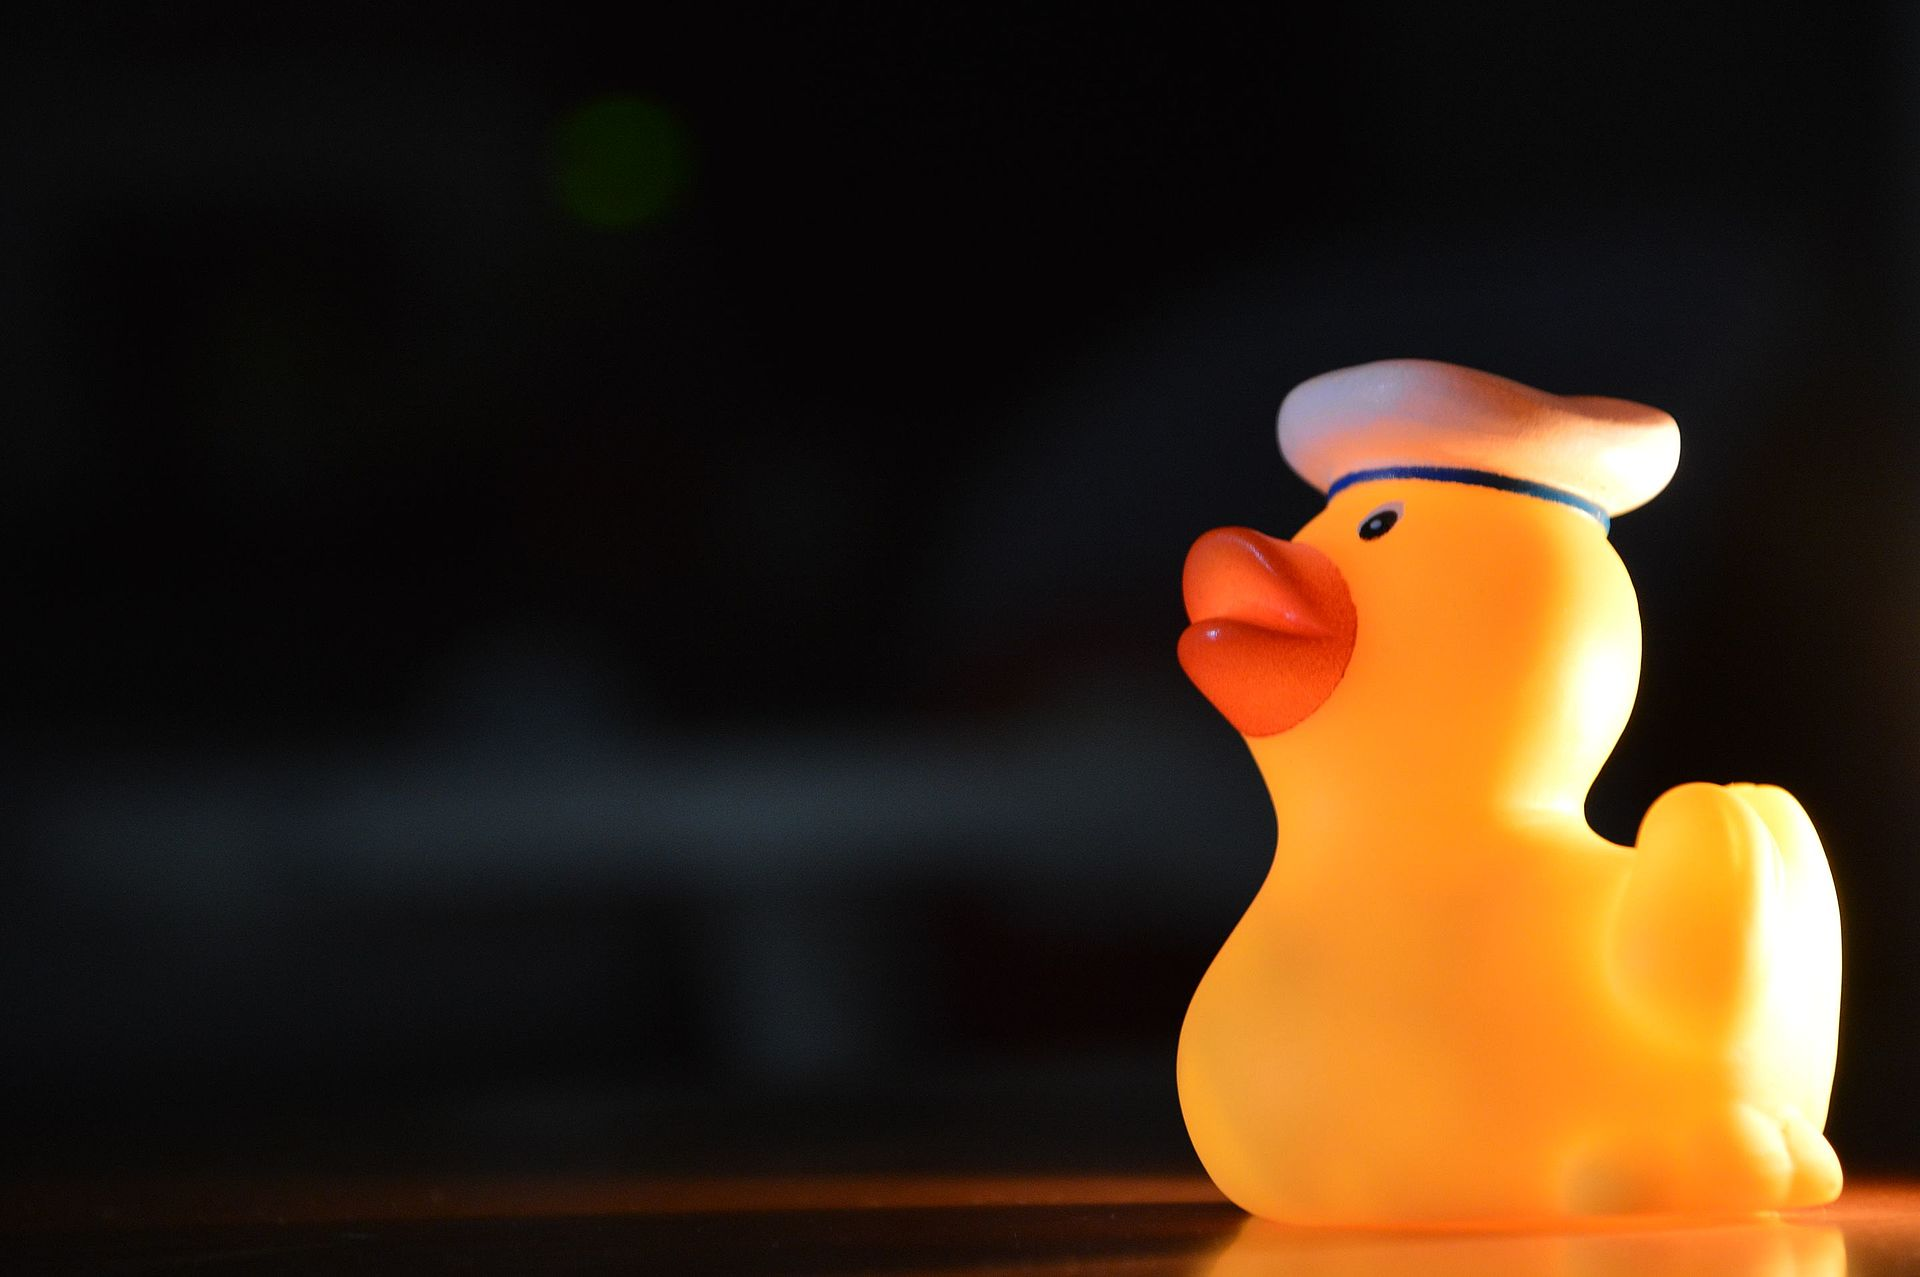
\includegraphics[width=0.5\textwidth]{Part_1/chapters/chapter_1/pictures/Rubber_duck.png}
            \caption{Un joli canard en plastique\label{Fig::rubberduck}}
        \end{wrapfigure}

        
        Et comme l'explique je sais pas qui dans le papier je sais pas quoi\cite{MNS}, les canards en plastique (voir Fig \ref{Fig::rubberduck}) ne sont absolument pas dangereux.
        
    \section{Les neutrinos et leurs oscillations}
        \subsection{Histoire de la découverte}
            \subsubsection{Première théorisation}
                énergie manquante dans je sais plus quelle expérience, on suppose nouvelle particule
            \subsubsection{Première observation}
                première mesure du neutrinos électronique
            \subsubsection{Deux saveurs en plus}
                Observations mu et tau et prédiction des neutrinos associés
                Observation des mu et tau
            \subsubsection{Oscillations}                
                Observation et premières interprétations (fin du monde et tout et tout)
                Théorisation
                nous verrons les détails plus tard
            \subsubsection{Le rôle des neutrinos dans les découvertes des bosons W et Z}
                Gargamelle et autres
        \subsection{Oscillation des neutrinos}
            mécaQ de base
            joli schéma à réaliser
            Histo de proba en fonction de L/E
            Implication pour SM
            
        \subsection{Possibles origines de la masse des neutrinos}
            \subsubsection{Mécanisme BEH pour les neutrinos}
            \subsubsection{Terme de masse de Majorana}
            \subsubsection{Mécanisme Seesaw}
            
        \subsection{Impact sur la leptogènes de la violation CP dans le secteur Leptonique}
        
        \subsection{Les différentes sources de neutrinos}
            \subsubsection{Artificiels}
                \paragraph{Réacteurs}
                \paragraph{Accélérateurs}
            \subsubsection{Naturels}
                \paragraph{Solaires}
                \paragraph{Supernov\ae}
                \paragraph{Géologiques}
                \paragraph{Big Bang}
    
\begin{subappendices}
    \section{Lagrangien de champ}\label{sec::field_basis}
    Il est important de noter qu'une particule quantique n'est plus décrite par une position à un temps donnée, mais par une amplitude de probabilité qui est présente partout dans l'espace temps et qui se propage comme une onde. Une onde étant décrite par un champ, il est important de parler de théorie classique des champs, afin d'avoir une idée de la forme de notre possible lagrangien. 
                
                Un champ -- à une dimension pour commencer -- peut être modélisé par $n$ masses $m$ identiques reliés entre elle sur une ligne par des ressorts de raideur $k$ espacé par une distance $a$. L'énergie potentielle entre la masse $i$ et la masse $i+1$ est classiquement \bs V_i=\frac{1}{2}k(\phi_{i+1}-\phi_i)^2\es, et l'énergie cinétique de la masse $i$ est \bs T_i=\frac{1}{2}m \partial_t \phi_i^2 \es, où $\phi_i$ est le déplacement de la masse $i$ par rapport à sa position d'équilibre $x_i$. Le lagrangien total s'écrit alors 
                \be 
                    L=\sum\limits_{i=1}^n \left( \frac{1}{2}m \partial_t \phi_i^2\right) - \sum\limits_{i=0}^n \left( \frac{1}{2}k(\phi_{i+1}-\phi_i)^2 \right)
                \ee
                Commençons par montrer que $\phi$ décrit une onde. Pour ce faire, utilisons l'équation d'Euler-Lagrange \eqref{eq::EL} : 
                \beq 
                    \frac{\partial L}{\partial \phi_i} - \frac{d}{dt}\frac{\partial L}{\partial \partial_t \phi_i}=0 \nonumber \\
                    \Rightarrow \ddot{\phi}_i-\frac{k}{m}(\phi_{i+1}-2\phi_i+\phi_{i-1})=0
                \eeq
                %Il est possible de montrer (Annexe \ref{sec::demo_dispersion}) que, si $\omega^2=\frac{2k}{m}(1-cos(ka))$, des solution en ondes sont autorisées, de la forme :
                %\be 
                 %   \phi_i=A.cos(kx_i-\omega t)
                %\ee
                
                
                %Nous savons maintenant que l'amplitude $\phi$ peut être une onde. 
                Le prochain travail est d'étudier le lagrangien précédent dans la limite du continue. Faisons d'abord apparaître le module d'Young\footnote{Comme nous travaillons à une dimension, il n'y a pas de \textit{section} à proprement parler et le module d'Young s'écrit alors $Y=LF/dL$ où $L$ est la longueur à vide (ici $a$), $F$ est la force (ici $k(\phi_{i+1}-\phi_i)$) et $dL$ est l'allongement (ici $\phi_{i+1}-\phi_i$). Il se réduit donc à $ka$.} $ka$ ainsi que la densité massique $m/a$ :
                \be 
                    L=\sum\limits_{i=1}^n \left( \frac{1}{2}a\rho (\partial_t \phi_i)^2\right) - \sum\limits_{i=0}^n aY  \frac{1}{2}\left(\frac{\phi_{i+1}-\phi_i}{a}\right)^2
                \ee
                Nous pouvons à présent faire tendre $a$ vers $0$ et $n$ vers l'infini pour passer au continue. Nous considérons maintenant une distribution uniforme de masse, et nos positions discrètes $\phi_i$ deviennent une variable continue de la position $\phi(x)$. De plus, le terme en $\frac{\phi_{i+1}-\phi_i}{a}$ devient $\partial_x \phi$. Nous factorisons par $\rho$ en définissant le terme $c=\sqrt{\frac{Y}{\rho}}$, le lagrangien devient donc : 
                \beq \label{eq::lagrangien_fields}
                    L=\frac{1}{2}\int\limits_{0}^l\left( \rho (\partial_t \phi)^2 - Y (\partial_x \phi)^2 \right)dx \nonumber \\
                    =\frac{\rho}{2}\int\limits_{0}^l\left( (\partial_t \phi)^2 - c^2 (\partial_x \phi)^2 \right)dx 
                    %=\frac{\rho}{2}\int\limits_{0}^l \partial_{\mu}\phi \partial^{\mu} \phi. dx
                \eeq
                L'Annexe \ref{sec::EL_field} montre comment dériver les équations d'Euler-Lagrange pour un champ dont le lagrangien dépend de $\phi$, $\partial_{x}\phi$ et $\partial_{t}\phi$. Nous pouvons utiliser ces équations pour retrouver l'équation du mouvement de $\phi$ qui est :
                \beq
                    \partial^2_x \phi - c^2\partial^2_t \phi = 0
                \eeq
                Qui est l'équation de mouvement d'une onde se propageant à la vitesse $c$. Je tiens à souligner ici que l'analogie avec la propagation d'amplitude de probabilité ne doit pas être poussé trop loin. La vitesse $c$ peut avoir un sens mais la grandeur $\rho$, qui est la densité massique du milieu où se propage l'onde, n'en a pas : une amplitude de probabilité se propage dans le vide!
                
\printbibliography

    \section{L'étrange nature de la nature}\label{sec::strange_nature}
    
    Commençons par l'exemple type qui introduit la mécanique quantique : l'électron dans la double fente, illustré à la Figure \ref{Fig::double_slit}. La Figure \ref{Fig::double_slit_a} représente l'expérience des fentes d'Young\cite{young}, qui a mit en évidence le caractère ondulatoire de la lumière. En effet, comme l'illustre la Figure \ref{Fig::double_slit_b}, on peut faire l'analogie entre une onde de lumière et une onde à la surface de l'eau, où les creux et les bosses après les fentes créent une figure d'interférence. Il est important de noter ici que même si l'on envoi une \textit{seule onde} (une seule perturbation de la surface de l'eau), \textit{la figure d'interférence existe}. La lumière présentant les mêmes interférences, on en déduit qu'elle se comporte bien comme une onde.
                    
    Si l'on envoi des balles, i.e des particules classiques, (Figure \ref{Fig::double_slit_c}, on s'attend à avoir une distribution en forme de double fente sur le mur. Ce n'est pas ce que l'on observe quand on envoi des électrons. La Figure \ref{Fig::double_slit_d} montre le même résultats qu'avec des photons\cite{double_slit_electrons}, indiquant que les électrons aussi se comportent comme des ondes. Mais il est possible aussi d'envoyer des électrons un par un. Si l'on fait ceci, et si les électrons \textit{sont} des ondes, une figure d'interférence devrait être vue. Ce n'est pas le cas, comme le montre la Figure \ref{Fig::double_slit_e} : un seul point apparaît. Là où les choses se corsent, c'est si l'on envoi des électrons un par un pendant un moment, et qu'on laisse leurs traces à l'écran. Au bout d'un certain nombre de tir, on observe une figure d'interférence. Ceci n'a strictement aucune analogie classique correcte\footnote{La plus proche est celle de la bille en suspension sur de l'eau vibrante. Voir la vidéo de \textit{Veritasium} à ce sujet\cite{veritasium}.}. Et pour compliquer encore les choses, si l'on a un moyen de détecter par quelle fente passe l'électron, alors aucune interférence n'est observée.
                    
    L'interprétation faite de ce phénomène suit la théorie des probabilités. Il n'est pas possible de la \textit{comprendre}, au sens ou on ne peut la mettre en relation avec rien de notre expérience de notre vie de tous les jours, mais elle est en accord avec les observations à un tel point que plus personne ne doute de sa justesse aujourd'hui. L'idée est d'associer à chaque possibilité qu'a l'électron d'arriver en $x$ une amplitude de probabilité (un nombre complexe). L'électron n'a ici que deux possibilités, passer par la fente 1 ou par la fente 2, on nommes les amplitudes correspondantes $\phi_1(x)$ et $\phi_2(x)$. L'addition de ces amplitudes donne une troisième amplitude $\phi(x)$, dont on défini le carré de la norme que étant la probabilité de trouver l'électron en $x$. Tout ceci semble artificiel
    \section{L'invariance de jauge en électromagnétisme}\label{sec::EM_classique}

\begin{wrapfigure}{r}{0.5\textwidth}
    \be\label{eq::Max_1}
        \Vec{\nabla}.\Vec{B}=0 \text{ (Pas de monopôles magnétiques)} 
    \ee 
    \be\label{eq::Max_2} 
        \frac{\partial \Vec{B}}{\partial t} + \Vec{\nabla}\times \Vec{E}=\Vec{0} \text{ (Loi de Faraday)}
    \ee 
    \be\label{eq::Max_3}
        \Vec{\nabla}.\Vec{E}=\frac{\rho}{\epsilon_0} \text{ (Loi de Gauss)}
    \ee
    \be\label{eq::Max_4}
        \frac{\partial \Vec{E}}{\partial t}-c^2 \Vec{\nabla}\times \Vec{B} =-\frac{\Vec{j}}{\epsilon_0} \text{ (Loi d'Ampère)}
    \ee
    \caption{Les quatre équations de Maxwell}
\end{wrapfigure}

Le fait que les très célèbres équations de Maxwell (\eqref{eq::Max_1} à \eqref{eq::Max_4}) soient invariante sous une certaine transformation nous a permit dans la section \ref{sec::gauges} de créer une théorie de la physique des particules à bases de symétries de jauge locale, qui se sont révélées extrêmement fructueuse. Nous revenons un peu plus ici sur cette transformation et sur comment elle découle des équations de Maxwell.

La première chose que l'on remarque à propos de ces équations, c'est que ce sont des équations différentielles couplées. Deux d'entre elles font intervenir les variations de $\Vec{E}$ et $\Vec{B}$ simultanément. Nous allons donc chercher à "découpler" ces équations pour trouver une expression pour $\Vec{E}(\Vec{r},t)$ et une expression pour $\Vec{B}(\Vec{r},t)$. Nous tomberons naturellement sur la jauge de Lorenz. 

Prenons la première équation \eqref{eq::Max_1}. Le cours de licence de calcule différentielle nous a appris que le gradient d'un rotationnel est toujours nul. Nous écrivons donc 
\be \label{eq::B}
    \Vec{B}=\Vec{\nabla}\times \Vec{A}
\ee
Où $\Vec{A}$ est un champ vectoriel quelconque. En mettant ce résultat dans \eqref{eq::Max_2} nous obtenons : 
\be\nonumber
    \frac{\partial \Vec{\nabla}\times \Vec{A}}{\partial t} + \Vec{\nabla}\times \Vec{E}=\Vec{0}
\ee 
Les opérateurs de dérivations temporels et spatiaux commutent, nous pouvons donc factoriser de la manière suivante : 
\be
    \Vec{\nabla}\times \left(\frac{\partial \Vec{A}}{\partial t} +\Vec{E}\right)=\Vec{0}
\ee 
De la même manière que le gradient d'un rotationnel fait zéro, le rotationnel d'un gradient fait aussi zéro. Nous pouvons tenter une astuce similaire avec :
\be \label{eq::E}
    \frac{\partial \Vec{A}}{\partial t} +\Vec{E} = -\Vec{\nabla}.\phi
\ee 
Où $\phi$ est un champ scalaire quelconque.

Si l'on tenait \textit{vraiment} à isoler $\Vec{E}$ et $\Vec{B}$, on utiliserait à présent les deux dernières équations de Maxwell pour avoir les équations du mouvement de $\Vec{A}$ et $\phi$. Mais ce n'est pas le propos ici, vous pouvez vous reporter à n'importe quel cours d'électromagnétisme pour cela (j'ai un faible pour le premier chapitre des cours de Bjorn Felsager\cite{Felsager}). Nous allons plutôt constater ce qu'il se passe si l'on modifie les champs $\Vec{A}$ et $\phi$ de la manière suivante : 
\beq \label{eq::gauge_transf}
    \phi(\Vec{r},t) \rightarrow \phi(\Vec{r},t)+\frac{\partial \chi(\Vec{r},t)}{\partial t}\\
    \Vec{A}(\Vec{r},t) \rightarrow \Vec{A}(\Vec{r},t)-\Vec{\nabla}.\chi(\Vec{r},t)
\eeq
Avec $\chi$ un champ scalaire quelconque \textbf{dépendant éventuellement de $\Vec{r}$ et $t$} (je les ai mise exceptionnellement ici pour souligner ce point, mais je les enlève à nouveau dans la suite pour ne pas alourdir les notations). Les champs $\Vec{E}$ et $\Vec{B}$ en sont modifiés ainsi (en reprenant les équations \eqref{eq::B} et \eqref{eq::E}) :

\beq 
    \Vec{B}=\Vec{\nabla}\times\left(\Vec{A}-\Vec{\nabla}.\chi\right) \nonumber \\
    \Rightarrow \Vec{B}=\Vec{\nabla}\times\Vec{A}
\eeq 
Puisque le rotationnel d'un gradient est nul. On retombe donc sur l'équation \eqref{eq::B}. Il en va de même pour $\Vec{E}$ et l'équation \eqref{eq::E} :
\beq
    \Vec{E}=-\frac{\partial \left(\Vec{A}-\Vec{\nabla}.\chi\right)}{\partial t} - \Vec{\nabla}.\left(\phi+\frac{\partial \chi}{\partial t}\right) \nonumber \\
    \Rightarrow \Vec{E}=-\frac{\partial \Vec{A}}{\partial t}-\frac{\partial \Vec{\nabla}.\chi}{\partial t} - \Vec{\nabla}.\phi+\Vec{\nabla}.\frac{\partial \chi}{\partial t} \nonumber \\
    \Rightarrow \Vec{E} = -\frac{\partial \Vec{A}}{\partial t} -\Vec{\nabla}.\phi
\eeq

Ceci signifie que nous pouvons modifier nos champs $\Vec{A}$ et $\phi$ avec n'importe quel champ $\chi$ qui nous arrange sans changer la physique (puisque nous ne \textit{mesurons} pas ces champs). Un choix particulier de $\chi$ s'appelle un choix de jauge, les champs $\Vec{A}$ et $\phi$ sont les champs de jauges, et la transformation \eqref{eq::gauge_transf} est appelée transformation de jauge. Chaque choix peu amener à un résultat exploitable différent, mais nous n'en discuterons pas plus ici.

Passons à présent à la notation relativiste. En prenant pour convention le tenseur métrique 
\be 
    \eta_{\mu\nu}=
    \begin{pmatrix}
        1 & 0 & 0 & 0 \\
        0 & -1 & 0 & 0 \\
        0 & 0 & -1 & 0 \\
        0 & 0 & 0 & -1
    \end{pmatrix}
\ee 
le champ de jauge de l'électromagnétisme s'écrit 
\be
    A^{\mu}=(\phi,\Vec{A})
\ee 
en covariant et 
\be\label{eq::gauge_field}
    A_{\mu}=(\phi,-\Vec{A})
\ee 
en contravariant. La transformation de jauge s'écrit alors 
\be \label{eq::gauge_transf_relat}
    A_{\mu} \rightarrow A_{\mu}+\partial_{\mu}\chi
\ee 
Et c'est de là que démarre la section \ref{sec::gauges}.
    \section{Démonstrations diverses}

    \subsection{Equation d'Euler Lagrange en théorie des champs classiques}\label{sec::EL_field}
    
        Afin de retrouver l'équation d'Euler Lagrange, partons du lagrangien d'un champ classique s'étendant sur une dimension d'espace et le temps \eqref{eq::lagrangien_fields} :
        \be
           L=\int\limits_{x_1}^{x_2} \L(\phi,\dot{\phi},\partial_{x} \phi)dx
        \ee
        où $\L$ est défini comme la densité lagrangienne de champ. Nous avons rajouté une dépendance en $\phi$ au lagrangien pour prendre en compte un éventuel potentiel. L'action entre un temps $t_1$ et un temps $t_2$ s'écrit alors
        \be
           S(\phi)=\int\limits_{t_1}^{t_2}\int\limits_{x_1}^{x_2}\L dx dt
        \ee
        L'amplitude physique $\phi(x,t)$ est telle que l'action est minimisée, i.e une variation de $\phi$  de la forme \bs\phi'(x,t)=\phi(x,t)+\epsilon \eta(x,t)\es implique que 
        \be 
            \frac{dS}{d\epsilon}_{|\epsilon=0}=0
        \ee
        où le terme \bs\eta(x,t)\es s'annule en $t_1$, $t_2$, $x_1$ et $x_2$ (Figure \ref{Fig::path}). Ceci implique donc : 
        \beq\label{eq::EL_field}
           \int\limits_{t_1}^{t_2}\int\limits_{x_1}^{x_2}\frac{\partial \L}{\partial \phi'}_{|\phi} \eta + \frac{\partial \L}{\partial (\partial_{x} \phi')}_{|\phi} \partial_{x} (\eta) + \frac{\partial \L}{\partial (\partial_{t} \phi')}_{|\phi} \partial_{t} (\eta) .dx dt = 0 \nonumber \\
           \bullet \int\limits_{t_1}^{t_2}\int\limits_{x_1}^{x_2} \frac{\partial \L}{\partial (\partial_{x} \phi')}_{|\phi} \partial_{x} (\eta). d^3x dt = \int\limits_{t_1}^{t_2} \cancelto{0}{\left[ \frac{\partial \L}{\partial (\partial_{t} \phi')}_{|\phi} \eta \right]_{x_1}^{x_2}}dt - \int\limits_{t_1}^{t_2}\int\limits_{x_1}^{x_2} \partial_{x} \frac{\partial \L}{\partial (\partial_{x} \phi')}_{|\phi} \eta. dx dt \nonumber \\
           \bullet \int\limits_{t_1}^{t_2}\int\limits_{x_1}^{x_2} \frac{\partial \L}{\partial (\partial_{t} \phi')}_{|\phi} \partial_{t} (\eta). dx dt = \int\limits_{x_1}^{x_2} \cancelto{0}{\left[ \frac{\partial \L}{\partial (\partial_{t} \phi')}_{|\phi} \eta \right]_{t_1}^{t_2}}dx - \int\limits_{t_1}^{t_2}\int\limits_{x_1}^{x_2} \partial_{t} \frac{\partial \L}{\partial (\partial_{t} \phi')}_{|\phi} \eta. dx dt \nonumber \\
           \Rightarrow \int\limits_{t_1}^{t_2}\int\limits_{x_1}^{x_2} \left[\frac{\partial \L}{\partial \phi'}_{|\phi} - \partial_{t} \frac{\partial \L}{\partial (\partial_{t} \phi')}_{|\phi} - \partial_{x} \frac{\partial \L}{\partial (\partial_{x} \phi')}_{|\phi} \right] \eta .dx dt = 0 \nonumber \\
           \Rightarrow \textcolor{red}{\frac{\partial \L}{\partial \phi} - \partial_{t} \frac{\partial \L}{\partial (\partial_{t} \phi)} - \partial_{x} \frac{\partial \L}{\partial (\partial_{x} \phi)} = 0}
        \eeq
        Ce résultat, facilement généralisable à 3 dimensions d'espace, est l'équation d'Euler Lagrange en théorie des champs.
        
    \subsection{Retrouver le lagrangien d'un champ scalaire massif à partir de l'équation de Klein-Gordon}\label{sec::KG_lag}
        Il s'agit de comparer l'équation 
        \beq
            (P_{\mu}P^{\mu}-m^2)\phi=0 \nonumber \\
            -\partial_{\mu}\partial^{\mu}\phi - m^2\phi = 0
        \eeq
        à l'équation d'Euler-Lagrange \eqref{eq::EL_field}
        \be
            \frac{\partial \L}{\partial \phi} - \partial_{\mu} \frac{\partial \L}{\partial (\partial_{\mu} \phi)} = 0
        \ee
        Il suffit d'identifier \bs \partial_{\mu}\partial^{\mu}\phi \es à \bs \partial_{\mu} \frac{\partial \L}{\partial (\partial_{\mu} \phi)} \es et \bs -m^2\phi \es à \bs \frac{\partial \L}{\partial \phi} \es. En intégrant selon $\partial_{\mu}\phi$ et $\phi$ respectivement, on se retrouve avec une densité lagrangienne de la forme : 
        \be 
            \L=const_1 \left(\partial_{\mu}\phi\partial^{\mu}\phi-\frac{1}{2}m^2\phi^2\right) + const_2
        \ee
        Où $const_1$ et $const_2$ peuvent être choisies respectivement à 1 et 0 sans changer les équations d'Euler-Lagrange, et donc la physique. Le terme \bs \partial_{\mu}\phi\partial^{\mu}\phi \es est identifiable au terme de propagation d'un champ mécanique classique, et l'on voit apparaître en plus un terme de masse de la forme \bs m^2\phi^2\es. 
        

    \subsection{Formule relative à la relation de dispersion dans un champ classique}\label{sec::demo_dispersion}
        Nous partons de l'équation du mouvement pour une masse $m$ dans un réseau  de ressorts à 1 dimension :
        \be 
            \ddot{\phi}_i-\frac{k}{m}(\phi_{i+1}-2\phi_i+\phi_{i-1})=0
        \ee
        Et cherchons des solutions de la forme :
        \be 
            \phi_i=A.cos(kx_i-\omega t)
        \ee
        Ceci nous donne l'équation suivante :
        \be 
            A\omega^2 cos(kx_n-\omega t)+\frac{k}{m}A\big( cos(kx_{n+1}-\omega t)-2cos(kx_n-\omega t) + cos(kx_{n-1}-\omega t) \big)=0
        \ee 
        Commençons par utiliser $cos(a+b)=cos(a)cos(b)-sin(a)sin(b)$ pour séparer les $kx$ des $\omega t$ :
        \beq
            cos(kx_{n+1}-\omega t)-2cos(kx_n-\omega t) + cos(kx_{n-1}-\omega t)  \nonumber \\
            = cos(\omega t)\big(-2cos(kx_n)+cos(kx_{n+1})+cos(kx_{n-1})\big) \nonumber \\
            + sin(\omega t)\big(-2sin(kx_n)+sin(kx_{n+1})+sin(kx_{n-1})\big)
        \eeq
        Faisons de même pour séparer les $x_n$ et les $a$ dans $x_{n\pm 1}=x_n \pm a$  :
        \beq
            = cos(\omega t)\big(-2cos(kx_n)+cos(kx_n)cos(ka)+cos(kx_n)cos(ka) -sin(kx_n)cos(ka)+sin(kx_n)cos(ka) \big) \nonumber \\
            + sin(\omega t)\big(-2sin(kx_n)+sin(kx_n)cos(ka)+sin(kx_n)cos(ka) -sin(ka)cos(kx_n)+sin(ka)cos(kx_n) \big) \nonumber \\
        \eeq    
        \beq    
            =cos(\omega t)\big(cos(kx_n)(2cos(ka)-2)\big)\nonumber \\
            +sin(\omega t)\big(sin(kx_n)(2cos(ka)-2)\big)
        \eeq
        \be   
            =\big(2(cos(ka)-2)cos(kx_n-\omega t)\big)
        \ee
        et donc nous avons
        \be 
            A\omega^2 cos(kx_n-\omega t)+\frac{2k}{m}A\big((cos(ka)-1)cos(kx_n-\omega t)\big)=0
        \ee
        Il existe donc des solutions en onde si
        \be 
            \omega^2=\frac{2k}{m}\big(1-(cos(ka)\big)
        \ee
\end{subappendices}
\printbibliography